% Template for 61st conference for non-peer-reviewed articled
\documentclass[convention,peer-reviewed]{aesconf}

% Graphics path
\graphicspath{{./}{figs/}}

% UTF-8 encoding is recommended but use one that works for you.
\usepackage[utf8]{inputenc}

% Highly recommended package for better looking text automatically.
\usepackage{microtype}

% Natbib is used for more control on citations. You can use other moderd
% bibliography packages but please try to match the provided style.
\usepackage[numbers,square]{natbib} 


% These are useful for different purposes.
\usepackage{color}
\usepackage{url}
\usepackage{colortbl}
\usepackage{graphicx}
\usepackage{amsmath}
\DeclareMathOperator*{\argmin}{arg\,min}
\DeclareMathOperator*{\argmax}{arg\,max}
\usepackage{multirow}
\usepackage{rotating}
\usepackage{setspace}
\usepackage{subfigure}
\usepackage{svg}

% The full title of the paper
\title{Automatic Guitar Tablature Transcription from Audio using Inharmonicity Regression
and Bayesian Classification}

% Put the authors in order here. The number in brackets define the corresponding affiliation.
\author[1]{Jonathan J. Michelson}
\author[2]{Richard M. Stern}
\author[2]{Thomas M. Sullivan}

% Affiliations go here
\affil[1]{Electro-Harmonix / New Sensor Corporation}
\affil[2]{Department of Electrical and Computer Engineering, and School of Music, Carnegie Mellon University}

% Correspondece should include the corresponding author's name and e-mail address
\correspondence{Jonathan Michelson}{jon.michelson93@gmail.com}

% These are used for headers. Anything that fits is okay. Please use proper punctuation.

% If there are many authors, please use the form "First author et al."
\lastnames{Michelson et al.}

% Short title should describe your topic but not be too long.
\shorttitle{Tablature Transcription using Inharmonicity Regression}


% This is required and draws the top title
% AES top title. A little bit volatile but should work for now.
\savebox{\AEStop}{%
	\begin{minipage}{\textwidth}%
		\rule{\textwidth}{1.5pt}\\%
		\\%
		\begin{minipage}[c][\iftoggle{convention}{3.2cm}{3.7cm}][t]{0\textwidth}%
			\includegraphics[width=20mm]{./AESlogo.pdf}%
		\end{minipage}%
		\begin{minipage}{\textwidth}%
			\sffamily%
			\begin{center}%
				\LARGE Audio Engineering Society\\%
				\iftoggle{e_brief}{%
				\hspace{3mm}\fontsize{36}{38pt}\selectfont Convention e-Brief \AESEBriefNumber\\%
				}{%
				\iftoggle{convention}{%
				\fontsize{36}{38pt}\selectfont Convention Paper\\%
				}{%
				\fontsize{36}{38pt}\selectfont Conference Paper\\%
				}}%
				\vspace{0.2cm}%
				\large Presented at the \AESConferenceNumber \iftoggle{convention}{Convention\\}{Conference on\\}%
				\iftoggle{convention}{}{\AESConferenceTopic\\}%
				\AESConferenceDate, \AESConferenceLocation%
			\end{center}%
		\end{minipage}\\%
		\vspace{0.2cm}\\%
		\begin{minipage}{\textwidth}%
			\rmfamily\itshape\small	\AESLegalText%
		\end{minipage}\\%
		\\%
		\rule{\textwidth}{1.5pt}%
	\end{minipage}%
}

\begin{document}

\setlength{\parindent}{1em}

\twocolumn[
\maketitle % MANDATORY! 

\begin{onecolabstract}
We propose two new methods to classify guitar strings for automated tablature transcription using only monophonic audio. The first method estimates the linear regression of log-inharmonicities of guitar strings with respect to their pitches, and assigns unseen notes to the strings whose means and variances maximize the probability of their measured inharmonicities. The second method, developed as a baseline, characterizes the inharmonicity distribution of each fretboard position as a normal probability density, and then similarly assigns unseen notes to the fretboard positions that maximize the likelihood of their observed inharmonicities. Results from the standard Real World Corpus of guitar recordings show that exploiting regressions generally improves accuracy compared to our baseline, while both achieve adequate performance in guitar-independent test scenarios.
\end{onecolabstract}
]

\section{Introduction}
The guitar is a popular musical instrument whose family comprises a diverse collection of stringed instruments. Despite their variation, the majority of guitars have six strings tuned to $E2$ ($82$ Hz, String 6), $A2$ ($110$ Hz, String 5), $D3$ ($147$ Hz, String 4), $G3$ ($196$ Hz, String 3), $B3$ ($247$ Hz, String 2), and $E4$ ($330$ Hz, String 1). Most guitars also typically have upwards of 20 frets, allowing for versatile musical passage realizations along the fretboard. A consequence of the tuning and extensive fretting locations is  a substantial pitch overlap between neighboring strings; multiple fretboard locations can usually be selected to produce a given pitch. This ambiguity renders conventional music scores, which represent passages as notes and chords, undesirable for students trying to learn more skillful placement of scales and arpeggios, or for enthusiasts trying to uncover the fretboard positions used on riffs recorded by virtuosic players. Figure~\ref{fig:score-tabs} illustrates this ambiguity.  

Tablature is a popular alternative music notation that does not suffer from the one-to-many mapping of scores. The staff, instead of representing pitch as in classical notation, depicts a birds-eye view of the guitar neck from the perspective of the performer. Each of the six horizontal lines represents a corresponding string on the guitar, and numbers on each line specify the fret to be fingered. Reasons for tablature desirability are numerous \citep{macrae2010}, such as accessibility (legibility does not require formal musical training) and transportability (tablature can be easily represented with ASCII characters). 

Accurate tablature transcription is a laborious task. Dependable tablature containing few errors typically require the careful listening of a seasoned musician to an audio recording, and possibly video recordings for additional consultation. Reliable automation of this transcription task would benefit the guitar student community by expediting quality tablature generation and unearthing fretboard positions of guitar riffs in songs for which accurate tablature does not yet exist.
\begin{figure}[!t] 
\centering
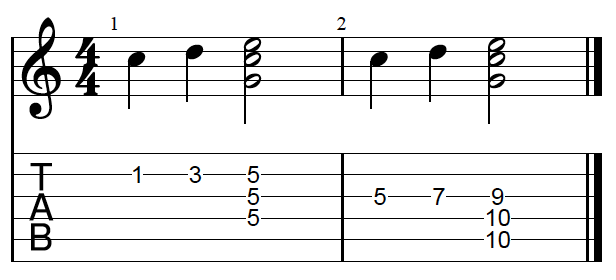
\includegraphics[width=70mm]{figs/score-tabs}
\caption{Two identical bars of a music score (top) and two equivalent realizations in tablature notation (bottom).}
\label{fig:score-tabs}
\end{figure}

An important feature in systems that transcribe tablature from audio is inharmonicity. When an ideal string fixed at both ends is displaced, the restoring force that causes it to oscillate is its tension. For a real string with stiffness, however, its elasticity contributes to this restoring force \citep{fletcher1962}, causing the frequencies of the modes of vibration to deviate from integer multiples of the fundamental. Instead, the solutions to the equation of motion of a string with stiffness and tension become: 
\begin{equation}
\label{eq:fk}
f_k = kf_{0}\sqrt{1+\beta k^2}
\end{equation}
where $f_k$ is the $k^{th}$ harmonic of fundamental $f_0$ and $\beta$ is the inharmonicity of the string, defined by
\begin{equation}
\beta = \frac{\pi^3 Q d^4}{64 T l^2}. \label{eq:beta}
\end{equation}
The inharmonicity $\beta$ of a vibrating string is a dimensionless quantity that depends on the Young's modulus $Q$, diameter $d$, tension $T$, and vibrating length $l$ of the string, and which skews the $k^{th}$ partial of the string upwards in frequency according to Eq.~(\ref{eq:fk}). See Fig.~\ref{fig:skew-freq}. 

\begin{figure}[!htbp]
\centering
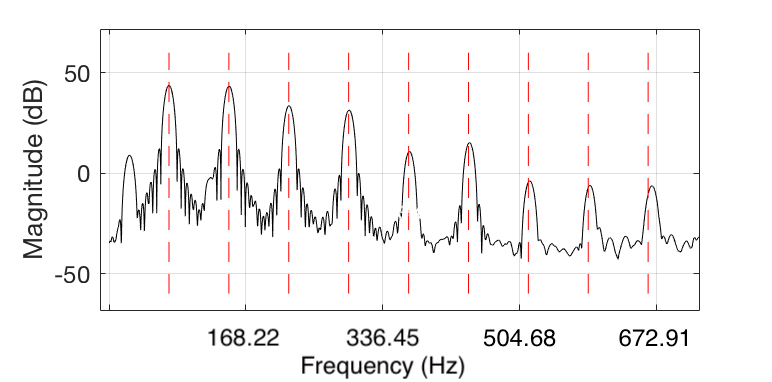
\includegraphics[scale=0.3]{skew-freq}
\caption{Power spectrum of note D2 plucked on an electric guitar at string 5 and fret 5. Red dashed lines are drawn at integer multiples of the fundamental. The partial peaks begin visibly skewing rightward after the fifth harmonic.}
\label{fig:skew-freq}
\end{figure}

Moreover, inharmonicity in the guitar varies in a deterministic manner with respect to fret positions along a given string \citep{barbanchoi2012}. Specifically, the inharmonicity $\beta(s,n)$ of a note produced by string $s$ at fret number $n$ can be expressed in terms of the inharmonicity of the open-string note $\beta(s,0)$ according to:
\begin{equation} 
\label{eq:beta-traj}
\beta(s,n) = \beta(s,0)2^{n/6}
\end{equation}
Figure~\ref{fig:beta-trajectories-ag} illustrates these theoretical trajectories. Barbancho \emph{et al.} \citep{barbanchoi2012} have developed a successful transcription system which exploits only these theoretical trajectories. We wondered, though, whether consideration of the \textit{empirical} inharmonicity trajectories could further increase accuracy; knowledge of the inharmonicity of every fret instead of only that of the open-string note could conceivably produce a more accurate picture of the inharmonicity trajectory, which could improve transcription performance.

We therefore propose classifying unknown notes by obtaining comprehensive log-inharmonicities of the notes along the guitar neck, estimating the string-wise linear regressions of these log-inharmonicities with respect to their pitches, and assigning the unknown notes to the strings whose regressions most probably predict the estimated log-inharmonicity of the notes. To contextualize its performance as well as that of the system developed by Barbancho \emph{et al.} \citep{barbanchoi2012}, we also introduce a baseline Bayesian classifier of fretboard position given an unseen note: the measured inharmonicities of each fretboard position are collected and fit to a normal distribution, and are used to return the string that maximizes the probability of having observed the measured inharmonicity of the unseen note.

\begin{figure}[t] 
\centering
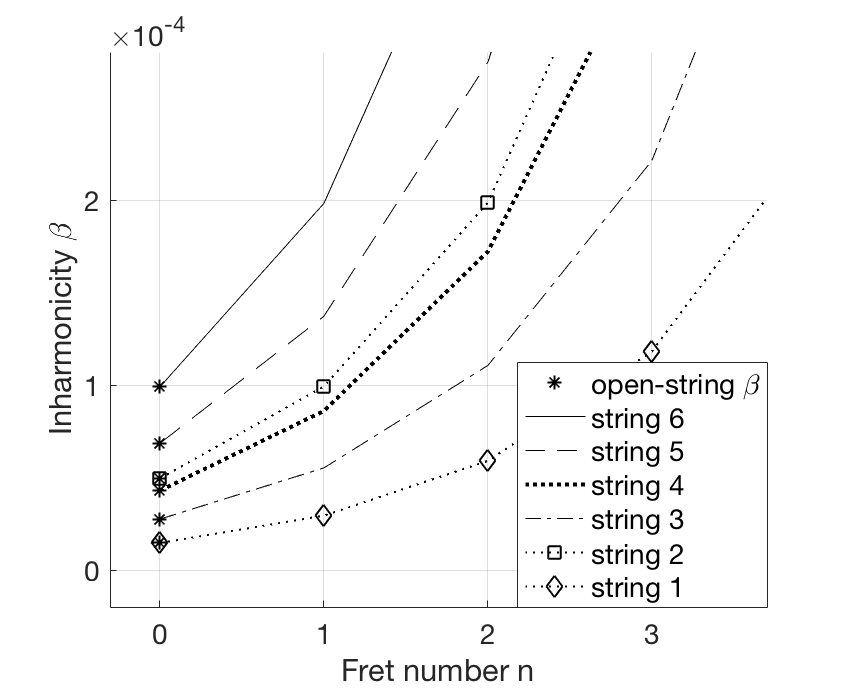
\includegraphics[scale=0.25]{figs/beta-trajectories-ag}
\caption{Example inharmonicity trajectories of acoustic guitar strings, calculated from measured open-string inharmonicities. Only Fret 0 (open-string) through Fret 3 are shown. On this acoustic guitar, the thinner Strings 1 and 2 were unwound while the thicker Strings 3-6 were wound, which helps explain the anomalous inharmonicity-trajectory location of String 2.}
\label{fig:beta-trajectories-ag}
\end{figure}


\section{Previous Work}

Empirical estimation of inharmonicity has been investigated for nearly 40 years. The use of pitch extraction techniques to perform estimation was first attempted by Galembo in 1979 and 1986 \citep{galembo1979,galembo1987}. In 1994, Galembo \emph{et al.} hypothesized a connection between partials-based fundamental pitch estimates and the degree of inharmonicity in a spectrum \citep{galembo1994}. The same authors subsequently  introduced another method in 1999 based on inharmonic comb filters \citep{galembo1999}. Rauhala  introduced an efficient iterative procedure in 2007 \citep{rauhala2007}, and two years later Hodgkinson  improved on its efficiency and accuracy with the median-adjustive trajectories (MAT) method \citep{hodgkinson2009}.

Inharmonicity-based tablature transcription from audio has also been the subject of ample study. In 2012, Barbancho \emph{et al.} introduced a transcription scheme based solely on inharmonicity analysis \citep{barbanchoi2012}. We refer to their work as the partial coincidence tally (PCT) method. In the following two years, Abesser \citep{abesser2012}, Kehling \citep{kehling2014}, and Dittmar \citep{dittmar2013} developed machine learning-based transcription systems that used slews of features which included inharmonicity.

This paper builds on the exclusively inharmonicity-based previous work in \citep{barbanchoi2012} by considering the inharmonicity of every fret in its estimation of the trajectory instead of only that of the open-string note, and by introducing a baseline likelihood-maximizing method against which to benchmark transcription performance.

\section{Methods}

\subsection{Inharmonicity Regression}
\label{sub:inharmonicity-regression}
Our approach begins with an estimation of the inharmonicity of an unseen note. The algorithm we employed was the median adjustive trajectories (MAT) method \citep{hodgkinson2009} proposed by Hodgkinson in 2009. The MAT algorithm was chosen for its efficiency and accuracy over the algorithms that preceded it \citep{hodgkinson2009}. We applied this estimation procedure to five Hann-windowed, 44.1-kHz audio segments of length $2^{14}$ samples, beginning at the detected onset of a note and at four successive 100-ms intervals (\emph{i.e.} 0 ms, 100 ms, 200 ms, 300 ms, and 400 ms after the note onset). This yielded five inharmonicity estimates that we later compiled into one classification result using the frame-aggregation refinement technique described in \citep{abesser2012}.

Next, we applied a log transformation to the estimated inharmonicities to make their variation linear with respect to MIDI pitch. Reconsidering Eq.~\eqref{eq:beta-traj} in terms of MIDI pitch number $m$ instead of fret number $n$, we obtain
\begin{equation}
\beta(s,m) = \beta(s,m_{os})2^{(m-m_{os})/6},
\end{equation}
where $m_{os}$ is the open-string pitch of string $s$. Figure~\ref{fig:beta-v-midi} illustrates these trajectories in terms of MIDI pitches.

\begin{figure}[!t] 
\centering
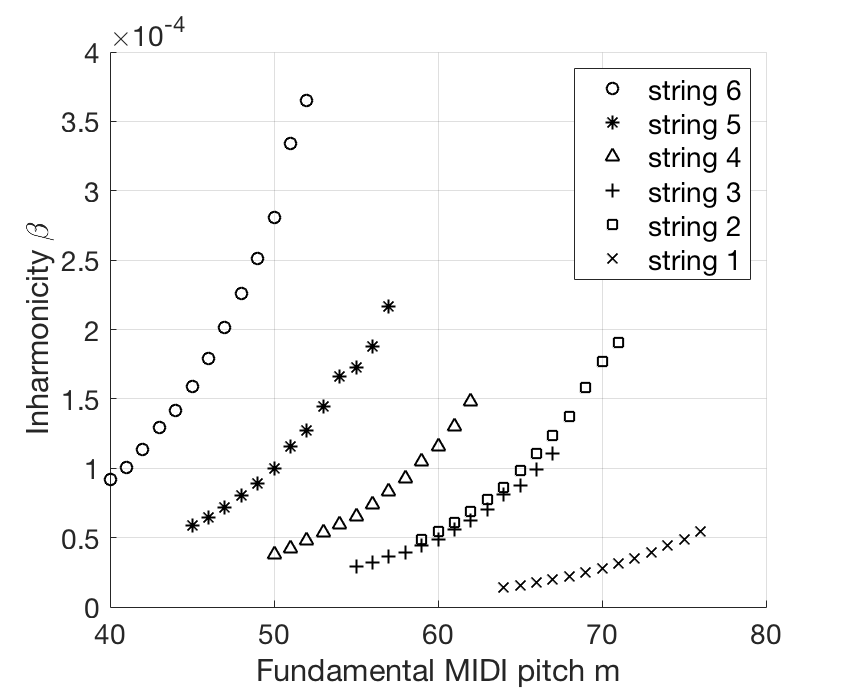
\includegraphics[scale=0.25]{beta-v-midi}
\caption{Inharmonicity estimates for Frets 0-12 on Strings 1-6 of RWC Acoustic Guitar AG111, plotted against MIDI fundamental instead of fret number.}
\label{fig:beta-v-midi}
\end{figure}

Considering  the log-inharmonicity $\beta_{l}(m)$, we see that
\begin{equation}
\beta_l(m) = \log_2\beta(s,m) = \log_2[\beta(m_{os})2^{(m-m_{os})/6}]
\end{equation}
\begin{equation}
\beta_l(m) = \log_2\beta(m_{os}) + (m-m_{os})/6
\end{equation}
\begin{equation}
\beta_l(m) = (\log_2\beta(m_{os})-m_{os}/6) + (1/6)m,
\end{equation}
where string $s$ has been dropped from the notation since we are looking only at variation along a fixed string. Substituting $w_0$ for $\log_2\beta(m_{os})-m_{os}/6$ and letting $w_1 = 1/6$, we obtain the standard linear form
\begin{equation}
\label{eq:linear-traj}
\beta_l(m) = w_0 + w_1m,
\end{equation}
which shows that the log-inharmonicity trajectory of a given string varies linearly with respect to both MIDI pitch and fret number, as seen in Fig.~\ref{fig:log-beta-v-midi}.

We next used linear regression to obtain empirical log-inharmonicity trajectories. We collected all notes with common string labels in our training data and performed linear regression of their log-inharmonicities $\beta$ against their fundamental pitches $m$ (in MIDI note number format), repeating  this procedure  for each string label. 

\begin{figure}[!t] 
\centering
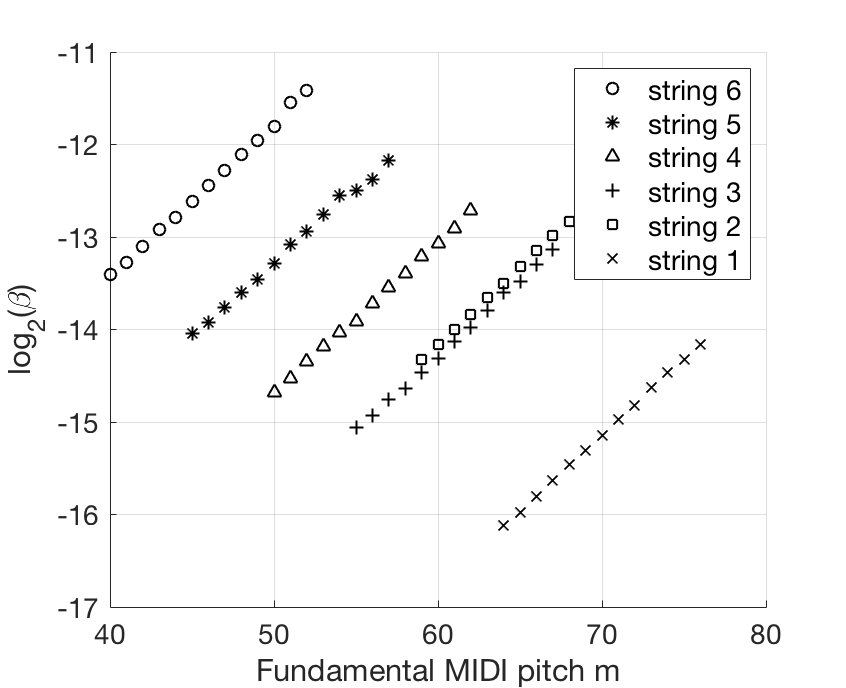
\includegraphics[scale=0.25]{log-beta-v-midi}
%\includesvg{figs/log-beta-v-midi}
\caption{Log-inharmonicity estimates for the same frets, strings, and guitar as Fig.~\ref{fig:beta-v-midi}.}
\label{fig:log-beta-v-midi}
\end{figure}

Let $s \in \{1,2,3,4,5,6\}$ be the string label to which each training note is assigned, and $N_s$ be the number of notes we have belonging to string label $s$. If we let $\mathbf{x}_s^{(i)} = [1, m_s^{(i)}]^T$ represent the $i^{th}$  note with fundamental pitch $m^{(i)}_s$ belonging to string $s$ , and let $\beta_s^{(i)}$ denote the log-inharmonicity of the $i^{th}$ note belonging to string $s$, we can solve
\begin{equation}
\label{lin-reg}
\mathbf{w}_s = \argmin_{\mathbf{w}}{\sum_{i=1}^{N_s}{(\beta^{(i)}_s - \mathbf{w}^T\mathbf{x}^{(i)}_s)^2}}
\end{equation}
which yields the weight vector $\mathbf{w}_s$ that minimizes the sum of squared error between the measured and predicted inharmonicities of the notes belonging to string $s$.
%\begin{figure}[!htbp] 
%\centering
%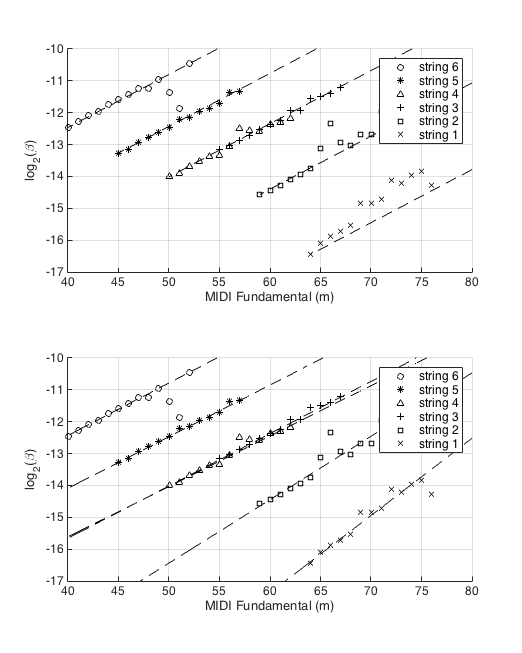
\includegraphics[scale=0.75]{traj-v-reg}
%\caption{Comparison of string inharmonicity characterization approaches for our recorded Fender Telecaster. Top: \textit{theoretical} trajectories. Note how each line begins precisely at the first marker of each string (i.e. the open-string note) and continues along a trajectory that ignores empirical inharmonicity estimates. String 1 most clearly shows this. Additionally, the trajectories for String 3 and String 4 are effectively co-linear and therefore indiscriminable. Bottom: regressions, or \textit{empirical} trajectories. Each regression was obtained by minimizing the bisquare weighted error of the residuals of the string, so the lines more closely follow the empirical inharmonicity scatterplot estimates.}
%\label{fig:traj-v-reg}
%\end{figure}

Occasional estimates from the inharmonicity measurement routine were outliers that deviated substantially from the linear trajectory model, so instead of the standard unweighted regression in~\eqref{lin-reg} we performed a bi-square weighted linear regression to approximate the log-inharmonicities. Bi-square weighting is a robust linear regression procedure that minimizes a \textit{weighted} sum of squares which de-emphasizes outliers \citep{matlab-robustfit}. This provided us with higher-quality regressions that were more robust to stray inharmonicity measurements.

To classify unknown notes, we imposed Gaussian probability distributions over the inharmonicity measurements of each string centered at their trajectories, and evaluated them at the inharmonicities of unseen notes to determine the most likely string from which it came. The means of the Gaussians are the log-inharmonicity values of points on the line, and the variances of the Gaussians are those of the residuals of the regressions, $\sigma_s^2$. In this manner, the probability distribution that characterized the inharmonicity trajectory $\mathbf{w}_s$ of string $s$ at the fundamental pitch $m_0^{(i)}$ of the $i^{th}$ note $\mathbf{x}^{(i)} = [1,m_0^{(i)}]^T$ was defined as the normal distribution $\mathcal{N}(\mu, \sigma^2)$, with mean $\mu = \mathbf{w}_s^T\mathbf{x}^{(i)}$ and variance $\sigma^2 = \sigma_s^2$. Now to classify the $n^{th}$ unseen note $\mathbf{x}^{(n)}$, we measured its log-inharmonicity $\beta^{(n)}$ and obtained the probability that this log-inharmonicity was observed given each string $s$ according to
\begin{equation}
P(\mathbf{x}^{(n)},\beta^{(n)} | s) = \mathcal{N}(\beta^{(n)} | \mathbf{w}_s^T\mathbf{x}^{(n)},\sigma_s^2),
\end{equation}
and returned the predicted string $\hat{s}^{(n)}$ that maximized this probability,
\begin{equation}
\hat{s}^{(n)} = \argmax_{s}P(\mathbf{x}^{(n)},\beta^{(n)} | s).
\label{eq:string-argmax}
\end{equation}
We also attempted classification using a decision function that selected the trajectory which minimized the residual instead of maximizing the probability, but we found that the latter method performed better.

It was straightforward to transform the string classifier output into tablature notation because it was assumed the tuning $\mathbf{t} = [m_1, m_2, m_3, m_4, m_5, m_6]^T$ of the unknown guitar was known, where $m_s$ is the MIDI pitch number of the open note on string $s$. Since we had an estimate of the MIDI pitch $m^{(n)}$ of the $n^{th}$ unknown note, taking the difference between $m^{(n)}$ and the open pitch $m_s$ of its assigned string yielded the fret on which the note was played.

Finally, we refined the fretboard estimates with plausibility filtering \citep{abesser2012}, in which we rejected and reassigned string decisions that were implausible given the constraints and assumptions of the data. If our systems assigned to a note a string on which the corresponding fretted position was negative, it would be clear that a mistake was made since frets cannot possibly be lower than 0 (the open string). Similarly, if our system assigned to a note a string on which the corresponding fret is greater than 12, a mistake would have been made because our guitar recordings feature only frets 0-12. When either of these situations arose, we rejected the string classification decision and selected the next most probable string. If the succeeding string was also implausible, the process was iterated until all six strings were considered.

\subsection{Baseline Bayesian Classifier}
The hypothesis of our regression method was that exploitation of the linear trajectories of log-inharmonicities is helpful for transcription. To objectively evaluate this we developed a baseline classifier, which we simply called Bayesian classification, which \textit{did not} leverage                    the inharmonicity trajectories and whose results served as a benchmark.

As before, we first measured the inharmonicities of guitar notes using median-adjustive-trajectories (MAT). Frame aggregation was performed using the same specifications discussed in Section~\ref{sub:inharmonicity-regression}. Next, we estimated the inharmonicity distribution of each fretboard position $f$. For each of the $F=78$ positions (13 notes $\times$ 6 strings), we calculated the median $\tilde{\beta}_f$ and variance $\sigma^2_f$ of its inharmonicities, and used these to parameterize a Gaussian probability density $\mathcal{N}_f(\tilde{\beta}_f,\sigma^2_f)$. We chose the median to lessen the influence of outliers.

We then classified unseen notes. We measured the inharmonicity $\beta^{(i)}$ of the $i^{th}$ unseen note $\mathbf{x}=[1,m_0^{                                                                                                                                                                                                                                                                                                                                                                                                                                                                                                                                                                                                                                                                                                                                                                                                                                                                                                                                                                                                                                                                                                                                                                                                                                                                                                                                                                                                                                                                                                                                                                                                                                                                                                                                                                                                                                    }]^T$ with fundamental MIDI pitch $m_0^{(i)}$ and evaluated the probability $P_f(\beta^{(i)} | f) = \mathcal{N}_f(\beta^{(i)} | \tilde{\beta}_f,\sigma^2_f)$ of it having been generated by the Gaussian distribution $\mathcal{N}_f$. We again used plausibility filtering to narrow our search space $f \in \{1,2,3,...,F-1,F\}$ of possible fretboard positions by considering just the positions $f \in \{f_{m,1},f_{m,2},...\}$ that agree with the fundamental frequency of the unseen note. For standard 
tuning, this is a maximum of only three positions. To classify a note, we selected the candidate fretboard position which maximized the likelihood of the measured inharmonicity of the note, just as in equation~\eqref{eq:string-argmax}:
\begin{equation}
\hat{f} = \argmax_{f\in\{f_{m,1},f_{m,2}...\}}P(\beta^{(i)} | f).
\label{eq:string-classification-mle}
\end{equation}

\section{Results}  
\subsection{RWC Transcription}
We evaluated our baseline and regression methods using a subset of the Real World Corpus (RWC) database \citep{goto2003}. The selected RWC recordings were isolated monophonic notes enumerating every fret on every string. We transcribed nine RWC guitars (three classical, three acoustic, and three electric) at three levels of context: guitar-specific, guitar-averaged, and guitar-independent. For guitar-specific trials, we trained and tested the system on the same guitar using three-fold cross-validation. For guitar-averaged trials, we trained the system on all recordings of the two guitars in the same class as the test guitar, as well as a two-thirds training portion of the test guitar, and then evaluated on the remaining third of the test guitar recordings. For guitar-independent trials, we trained the system on two of the guitars in the same class as the test guitar, and tested on all recordings of the remaining one. We used error probabilities to quantify the transcription performance for each guitar.
%\twocolumn[
%\maketitle

Figure~\ref{fig:novel-methods-sig-comp} compares the error probabilities and significance ($\alpha = 0.05$, McNemar test \citep{McNemar1947}) of our two novel methods in all three contexts. Figure~\ref{fig:sig-comp-PCT} compares the error probabilities and significance ($\alpha = 0.05$, $t$-test) of our methods and the PCT method developed in \citep{barbanchoi2012}. Because we did not have access to the trial-by-trial transcription results of PCT, we approximated the standard deviation $\sigma_d$ of the distribution of the differences by the square root of the average of the variances of the methods $\sigma_d = \sqrt{(\sigma^2_1+\sigma^2_2)/2}$ according to the Bernoulli approximation, in which $\sigma_x^2 = p_x(1-p_x)$ where $p_x$ is the probability of a correct classification for a given set of conditions.

\begin{figure}[!t]
\centering
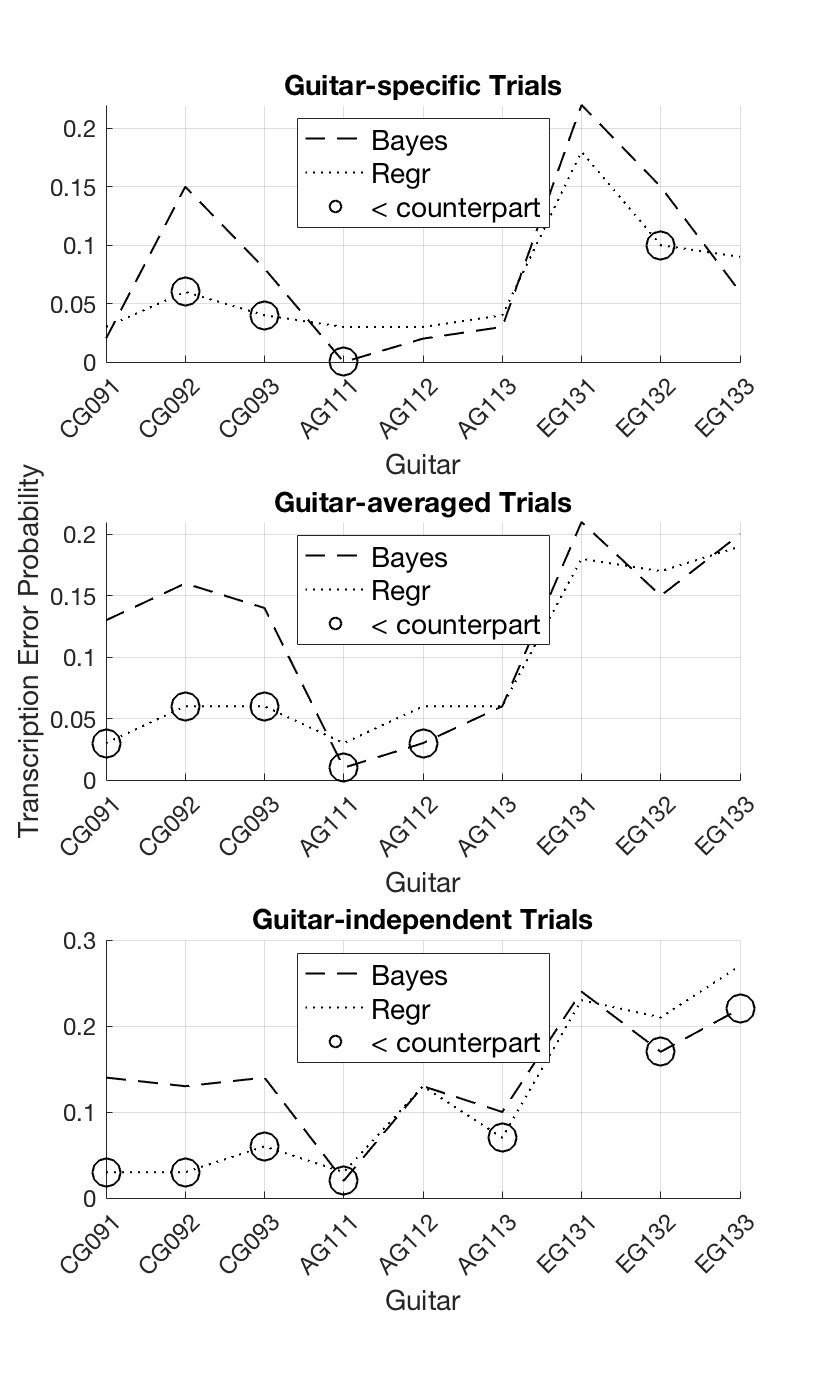
\includegraphics[scale=0.275]{novel-methods-sig-comp}
\caption{For each guitar, the method (Bayes or Regression), if either, that performed significantly better than its counterpart is marked with a circle.}
\label{fig:novel-methods-sig-comp}
\end{figure}

Lastly, Tables~\ref{tab:cg-str-f}, ~\ref{tab:ag-str-f}, and ~\ref{tab:eg-str-f} display the string-wise F1-scores of our regression method for each of the classical, acoustic, and electric guitars, respectively. The evaluation scenario from which these scores were tabulated was the ``Guitar-averaged" scenario. 

\begin{figure}[!t]
\centering
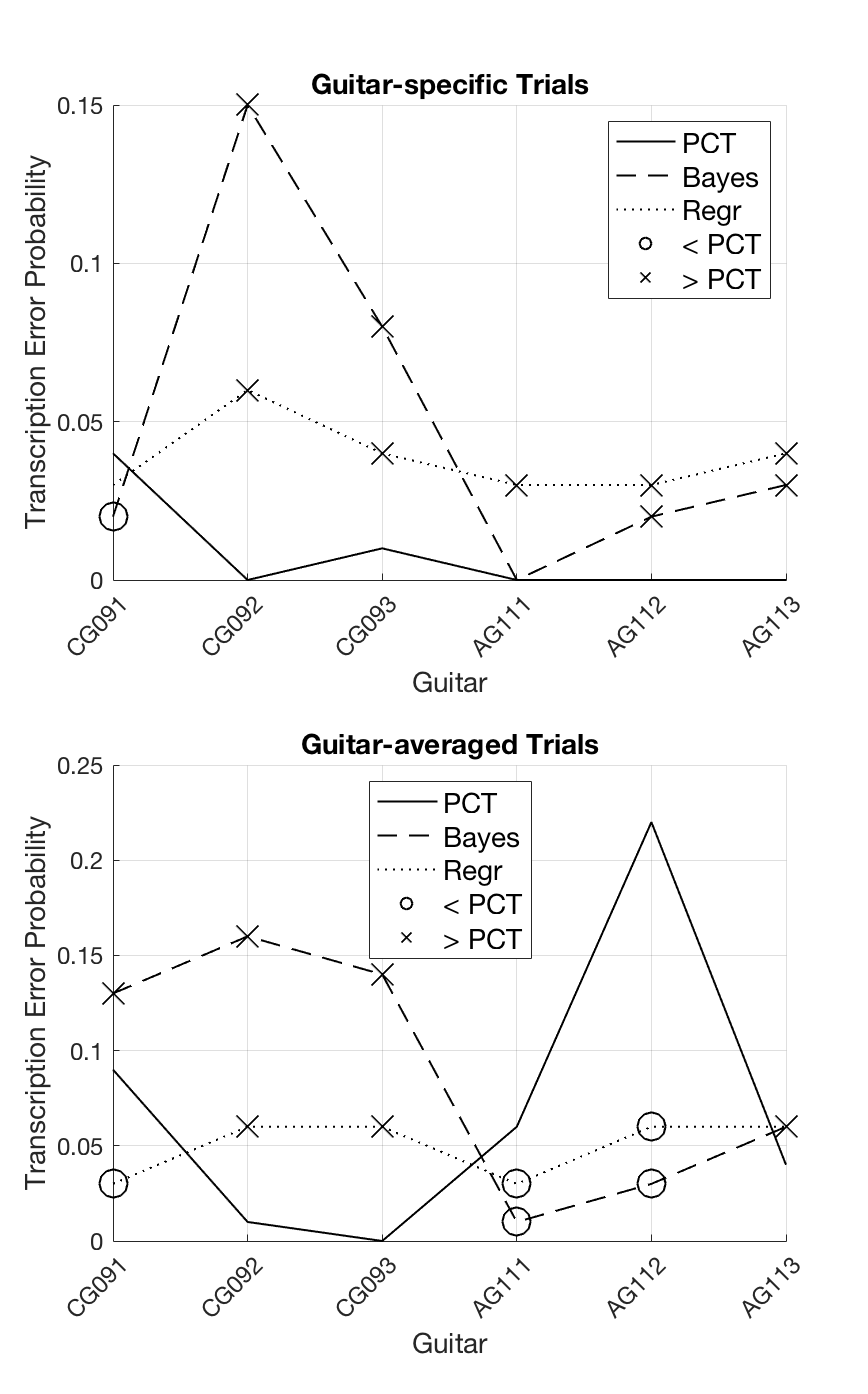
\includegraphics[scale=0.25]{sig-comp-PCT}
\caption{For each guitar, if our methods performed significantly differently than PCT we mark it with either an `O' or an `X'. The former denotes significantly lower error probability while the latter denotes significantly higher error probability.}
\label{fig:sig-comp-PCT}
\end{figure}

\begin{table}[!h]
\begin{center}
\begin{tabular}{||c|c|c|c|c||}
\hline
\multicolumn{5}{||c||}{\bf{Transcription F1-scores}} \\
\hline
String No. & CG1 & CG2 & CG3 & Overall CG \\
\hline
1 & 0.96 & 0.93 & 0.96 & 0.95\\
\hline
2 & 0.92 & 0.90 & 0.91 & 0.91\\
\hline
3 & 1.00 & 0.95 & 0.96 & 0.97\\
\hline
4 & 0.96 & 0.93 & 0.91 & 0.93\\
\hline
5 & 1.00 & 0.96 & 0.93 & 0.96 \\
\hline
6 & 1.00 & 0.98 & 1.00 & 0.99\\ 
\hline
\hline
\end{tabular}
\caption{String-wise F1-scores for the RWC classical guitars, using regression classification for the ``Guitar-averaged" scenario.} 
\label{tab:cg-str-f}
\end{center}
\end{table}

\begin{table}[!h]
\begin{center}
\begin{tabular}{||c||c|c|c|c||}
\hline
\multicolumn{5}{||c||}{\bf{Transcription F1-scores}} \\
\hline
String No. & AG1 & AG2 & AG3 & Overall AG \\
\hline
1 &  0.96 & 0.96 & 0.96 & 0.96 \\
\hline
2 & 0.94 & 0.80 & 0.87 &  0.87\\
\hline
3 & 0.91 & 0.89 & 0.85 & 0.88\\
\hline
4 & 1.00 & 1.00 & 0.99 &  1.00 \\
\hline
5 & 1.00 & 1.00 & 0.99 &  1.00 \\
\hline
6 & 1.00 & 1.00 & 1.00 & 1.00 \\ 
\hline
\hline
\end{tabular}
\caption{String-wise F1-scores for the RWC acoustic guitars, using regression classification for the ``Guitar-averaged" scenario.} 
\label{tab:ag-str-f}
\end{center}
\end{table}

\begin{table}[!h]
\begin{center}
\begin{tabular}{||c||c|c|c|c||}
\hline
\multicolumn{5}{||c||}{\bf{Transcription F1-scores}} \\
\hline
String No. & EG1 & EG2 & EG3 & Overall EG\\
\hline
1 & 0.96 & 0.94 & 0.96 & 0.95 \\
\hline
2 & 0.94 & 0.95 & 0.72 & 0.87\\
\hline
3 & 0.47 & 0.42 & 0.42 &  0.44\\
\hline
4 & 0.66 & 0.72 & 0.79 &  0.72\\
\hline
5 & 0.85 & 0.92 & 1.00 &  0.92 \\
\hline
6 & 0.96 & 0.98 & 1.00 &  0.98 \\ 
\hline
\hline
\end{tabular}
\caption{String-wise F1-scores for the RWC electric guitars, using regression classification for the ``Guitar-averaged" scenario.} 
\label{tab:eg-str-f}
\end{center}
\end{table}

\section{Discussion} 
\subsection{RWC Transcription}
Figure~\ref{fig:novel-methods-sig-comp} shows that in ten of the twenty-seven RWC classical, acoustic, and electric guitar trials, the regression approach significantly outperformed the Bayesian baseline. The Bayesian baseline provided better performance on six of the audio segments, and there was no significant difference between the two for the remaining eleven recordings. Overall this suggests there is some merit to exploiting the structure of log-inharmonicity trajectories for improved transcription.

The ``Guitar-independent Trials" plot of Figure~\ref{fig:novel-methods-sig-comp} shows that the transcription performance of both our regression and baseline methods for unseen guitars remains adequate, which suggests that our systems exhibit an appreciable degree of generalizability. It is unclear, however, whether this degree of generalizability is unique; while we would have liked to compare the performance of PCT and our methods in this trial context, ``guitar-independent'' results were not reported in \citep{barbanchoi2012}.

Figure~\ref{fig:sig-comp-PCT} shows that PCT performed at a level that was equal to or better than  our two methods in eight of the twelve RWC classical and acoustic trials. At the time of writing of this paper we were not sure whether the authors of PCT used the same subset of RWC electric guitars, so we omitted them from our analysis. While we had expected that prior consideration of the inharmonicity of every fret would help our classifier obtain a more reliable picture of the inharmonicity trajectory, it appears that this is not the case. The better performance of PCT suggests that the theoretical inharmonicity trajectories are sufficient for transcription, at least for the ``guitar-specific'' and ``guitar-averaged'' trial contexts of classical and acoustic guitars. 

The string-wise transcription performances in Tables~\ref{tab:cg-str-f}, ~\ref{tab:ag-str-f}, and ~\ref{tab:eg-str-f} provide further insight into our transcription error probabilities. The classical guitars overall exhibited reliable performance. For the acoustic guitars, however, the worst-performing strings were consistently String 2 and 3. This was expected given the proximity of their log-inharmonicity estimates in Figure~\ref{fig:log-beta-v-midi}. For the electric guitars, the worst-performing string was consistently String 3. It is possible that these acoustic and electric guitar string observations are partially due to patterns of variation in string geometry; on acoustic guitars, the decreasing thickness from String 3 to String 2 is typically accompanied by the absence of string winding. On electric guitars, the absence of winding can begin on either String 3 or String 2, depending on the string gauge.

To understand better the potential impact of guitar string geometry on estimated inharmonicity, we recorded identical note plucks on personal guitars exhibiting a wide variety of combinations of string age, intonation length, and gauge size, and winding.  We observed that variations in gauge size and winding affected our log-inharmonicity measurements by orders of magnitude between one-tenth and one, which is a degree of variability that is commensurate with differences between log-inharmonicity estimates for adjacent strings. The RWC database does not annotate string geometry parameters for any of its guitars, so it is possible that variations along these lines may have interfered with the quality of reported transcription results among systems using this database. We will explore the potential impact of this variability on our estimation quality in the future.

\section{Summary} 
Tablature is a popular music notation for guitarists because it uniquely specifies fretboard positions for musical passages. Its manual annotation process, however, is tedious. Automatic transcription systems offer a solution to this difficulty. Inharmonicity is a phenomenon which affects the degree of upward skew of the partials of a note, and it is a key feature used in many systems that attempt automated guitar tablature. We proposed capitalizing on the predictable log-inharmonicity trajectory of a string by characterizing it as a linear function of its pitch, and we developed a baseline Bayesian classifier that exploits this relationship. 

Comparisons between our baseline and regression methods suggested that exploiting inharmonicity regressions can be worthwhile, in that the regression-based approach achieved higher accuracy more frequently than the baseline did. The adequate transcription performance of the two methods in guitar-independent scenarios also suggested a degree of generalizability not reported in previous work. Nevertheless, our two approaches on average did not improve transcription accuracy on classical and acoustic guitars compared to the previously-developed PCT method in guitar-specific test scenarios. We also noted that guitar string geometry is an important factor to consider when developing inharmonicity-based methods, and our own results may have been better with more careful control of this variable.

\bibliographystyle{jaes}

% Reference to bibliography file.
\bibliography{mybib}


\end{document}